\section{Introduction}
\label{sec:introduction}

Researchers, students, and peer reviewers use document assistants to extract experimental results, definitions, and visual evidence from scientific PDFs. These documents are unusually difficult for question answering because a claim may depend on text, a table, a figure, or the spatial relationship between them. Existing retrieval-augmented generation (RAG) systems~\citep{lewis2020rag} can produce plausible answers, but following one citation back to the exact supporting region is still awkward, especially when an unpublished paper should remain on the reader's machine.

We demonstrate \textsc{SCHOLAR} as a concrete interaction: upload a paper, ask a question, receive a cited answer, click a citation, and inspect the corresponding paragraph, figure, or table region in the original PDF. The system keeps the evidence object---not merely a text snippet---attached to the answer and records retrieval, citation, verification, and final-output decisions in an audit trace.

\begin{figure}[t]
\centering
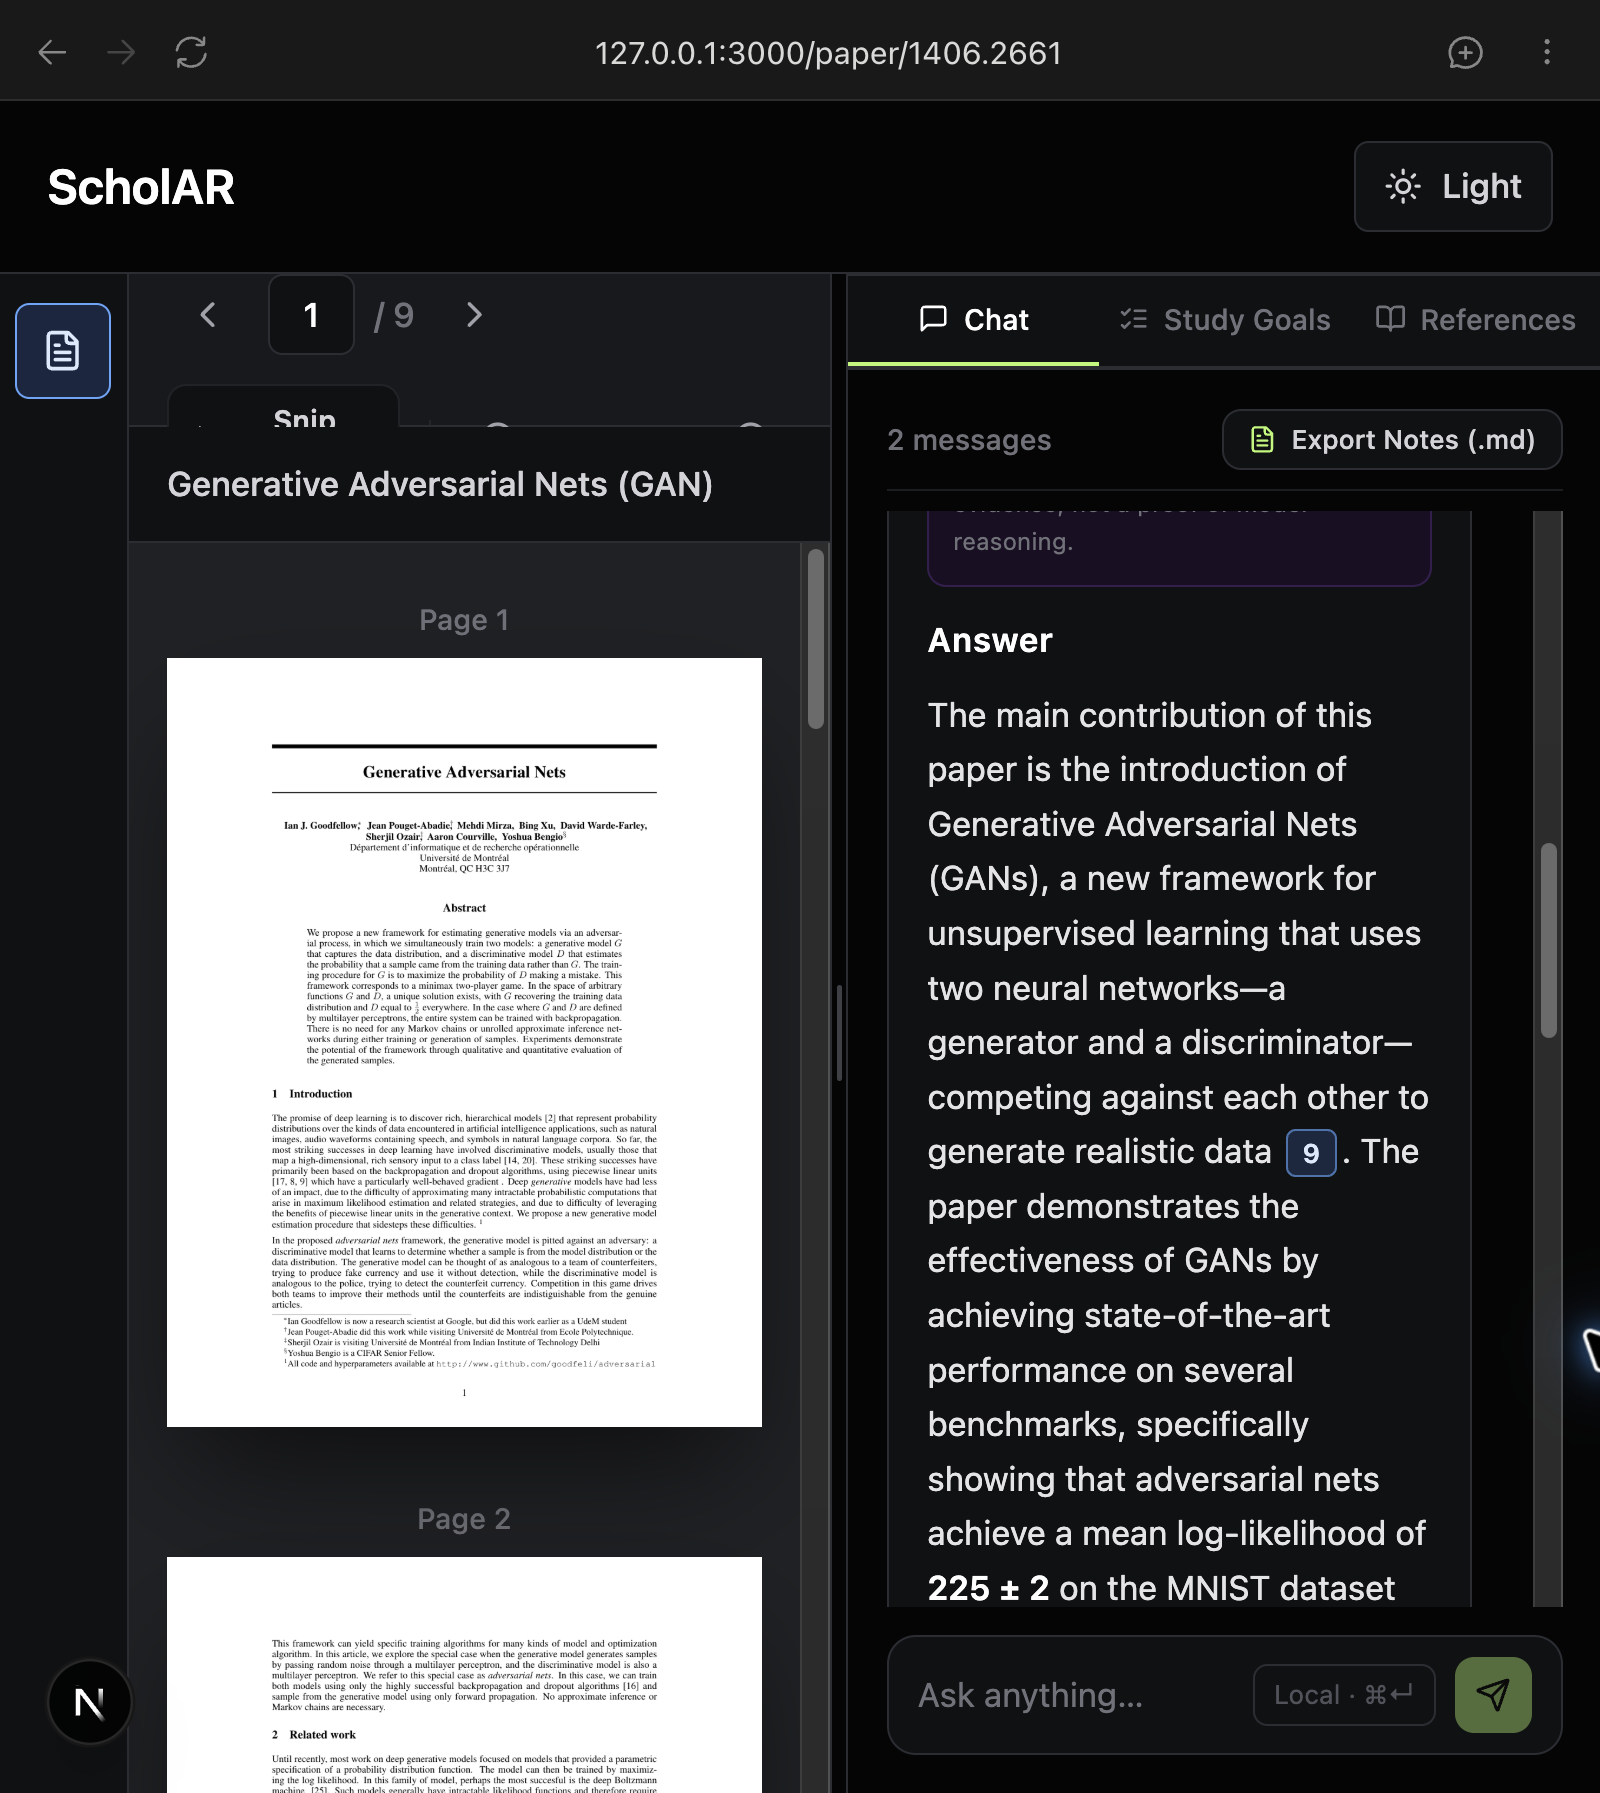
\includegraphics[width=\columnwidth,height=0.35\textheight,keepaspectratio]{figs/ui_demo.png}
\caption{\textbf{The interaction the demo exposes.} The workspace places the original PDF beside a cited answer; citation chips are the entry point to page and region inspection. The screencast shows the synchronized jump and evidence-inspection path.}
\label{fig:ui_demo_early}
\end{figure}

Scientific-document understanding benchmarks such as QASPER, SciFact, and M3SciQA show the need to retrieve and reason over scholarly evidence~\citep{dasigi2021qasper,wadden2020scifact,li2024m3sciqa}; citation-grounded generation studies examine whether retrieved context supports generated claims~\citep{gao2023alce,asai2024selfrag}; and multimodal document datasets show why page layout, figures, and tables matter~\citep{pramanick2024spiqa,faysse2025colpali}. Related EACL demonstrations address RAG evaluation and historical-manuscript analysis~\citep{es2024ragas,sakhovskiy2026inksight}. SCHOLAR differs in combining local execution with citations that retain spatial identity and can be inspected in the original PDF.

In this demonstration, we make three contributions:
\begin{enumerate}
    \item \textbf{Inspectable scientific QA:} A local-first assistant whose answer citations resolve to text bounding boxes, figures, and tables in the original PDF.
    \item \textbf{Auditable grounding pipeline:} Layout-aware document representation, hybrid retrieval, and deterministic lexical/numerical checks preserve the connection between generated claims and retrieved evidence.
    \item \textbf{Open interactive system:} A reproducible implementation characterized with retrieval, grounding, and consumer-workstation diagnostics, with the package and screencast supplied as submission artifacts.
\end{enumerate}

The software is MIT-licensed; access details are given in Section~\ref{sec:availability}.
